\documentclass[900pt, a0paper, landscape]{tikzposter}
\usepackage{etstikzposter}
\usepackage{tikz}
\usepackage{multirow} % Package for multirow tables
\usetikzlibrary{arrows, decorations.markings, arrows.meta, positioning} % TikZ libraries
\usepackage{overpic} % Overlay pictures
\usepackage{multicol} % Multiple columns
\usepackage[backend=biber]{biblatex} 
\addbibresource{main.bib} % Point to your .bib file
\usepackage{qrcode}
% Load Libertinus Math before fontspec
\usepackage{amsmath} % Essential for traditional math formatting
\usepackage{amssymb} % Provides additional math symbols
\usepackage{libertinus} % Libertinus for a more traditional math look

% Font settings
\usepackage{fontspec}
\usepackage{graphicx}
\usepackage{hyperref}
% Use Libertinus fonts for  both text and math
\setmainfont{Libertinus Serif} % Set Libertinus Serif as the main font
\setmathfont{Libertinus Math} 
\begin{document}
\maketitle
\node [text=titlefgcolor,
    outer sep=0pt,
    minimum width=\textwidth,
    minimum height=8cm,
    align=center,
    fill=titlebgcolor, inner sep=1mm] at (0,11) {
\hspace*{900pt}
\begin{minipage}[c][][c]{0.77\linewidth}
    \centering
    \fontsize{80}{90}\selectfont \textbf{Multi-person Physics-based Pose Estimation for Combat Sports}\\[4pt]
    \hspace*{-950pt}
    \fontsize{60}{80}\selectfont Hossein Feiz \quad David Labbé \quad Sheldon Andrews \\[2pt]
    \hspace*{-1410pt}
    \fontsize{30}{40}\selectfont École de technologie supérieure, Montréal, Québec, Canada
\end{minipage}

\hspace*{-1350pt}

\begin{minipage}[c][][c]{\linewidth}
    \centering
    
\includegraphics[height=5cm]{figures/podium.eps}
    \hspace*{40pt}
    
\includegraphics[height=4.5cm]{figures/ins.eps}
    \hspace*{40pt} 
    
\includegraphics[height=4.5cm]{figures/ets.eps}
    \hspace*{40pt}
    
\includegraphics[height=5cm]{figures/boxing.eps}
\end{minipage}

};


\begin{columns}
\column{0.5}
\block[titleoffsety=0.25cm, bodyoffsety=0.25cm]{Introduction}{
   \fontsize{36}{40}\selectfont Motion capture in sports scenes like boxing presents challenges due to occlusion, crowding, and fast movements. We used a multi-view setup requiring visibility from just two cameras. Our pipeline generates realistic motions using multi-person physics optimization while considering collisions between characters.}


\block[titleoffsetx=0cm, bodyoffsetx=0cm, titleoffsety=1cm, bodyoffsety=1cm]{Pipeline}{
\begin{overpic}[scale=3]{figures/pipeline.pdf}
\color{white}

\put(15.5,32){\rotatebox{-90}{\fontsize{22}{16}\selectfont Yolov8}}


\put(22.5,32){\rotatebox{-90}{\fontsize{22}{16}\selectfont XMem}}
\put(28,36){\rotatebox{-90}{\fontsize{22}{16}\selectfont Epipolar Constraints}}
\put(34,32){\rotatebox{-90}{\fontsize{22}{16}\selectfont ViTPose}}
\put(75,35.5){\fontsize{35}{17.5}\selectfont $\mathrm{L}_{\text{GMM}} + \, \mathrm{L}_{\text{Vposer}}$}
\put(18,8){\fontsize{25}{25}\selectfont Physics Body Model Generator}

\put(73,22.5){\fontsize{38}{15.8}\selectfont$\mathrm{L}_\text{2D}+ \mathrm{L}_\text{3D} + \mathrm{L}_{\beta}  $}
\put(63,1.3){\fontsize{36}{16}\selectfont$\mathrm{L}_\text{p,t}+ \mathrm{L}_\text{v,t} + \mathrm{L}_{\text{collision,t}}  $}

\color{black}
\put(18.5,35){\rotatebox{-90}{\fontsize{22}{16}\selectfont $\mathbf{bboxes}$}}
\put(36.5,32){\rotatebox{-90}{\fontsize{22}{16}\selectfont $\mathbf{J}_\text{2D}$}}
\put(66,32.5){\rotatebox{-90}{\fontsize{22}{16}\selectfont $\mathbf{J}_\text{3D}$}}
\put(70.5,29.5){\fontsize{30}{25}\selectfont Kinematics Optimization }
\put(59,8){\fontsize{27}{25}\selectfont Multi-person Dynamics Optimization }
\put(15,39){\fontsize{20}{20}\selectfont Multi-frame Multi-view Tracking IDs}
\put(74,14){\fontsize{40}{16}\selectfont $\mathbf{q} , \mathbf{v}, \mathbf{p}$}


\put(41,39){\fontsize{20}{20}\selectfont Weighted Triangulation and Filtering

}
\put(0.5,20){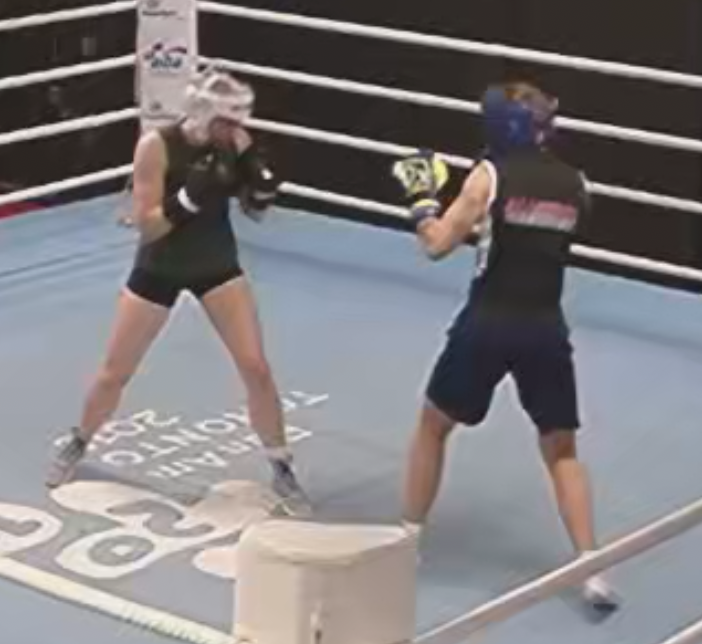
\includegraphics[scale=0.36]{figures/p1.png}} 
\put(0.5,32){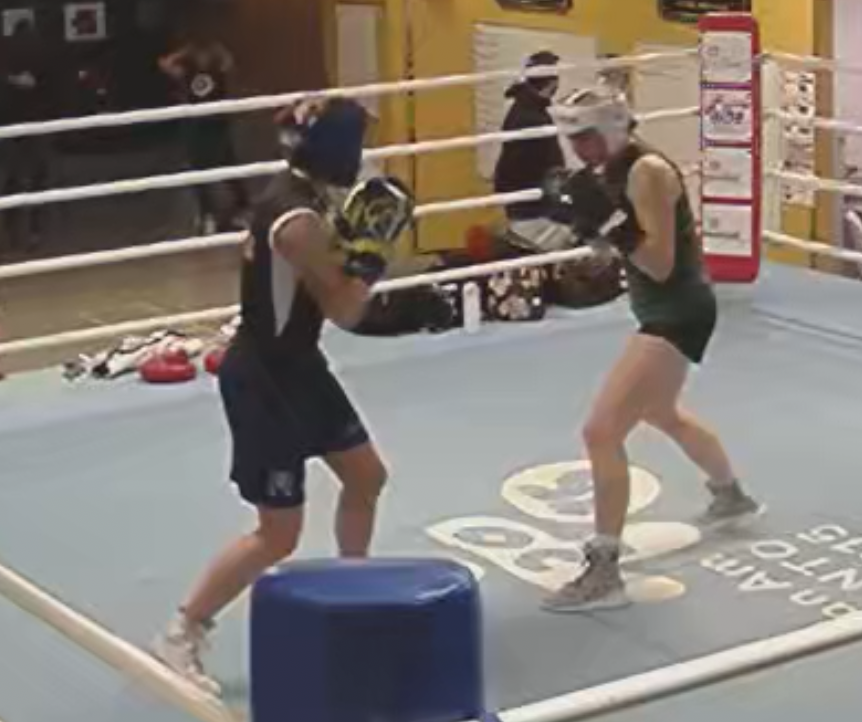
\includegraphics[scale=0.3]{figures/p2.png}}
\put(95,23){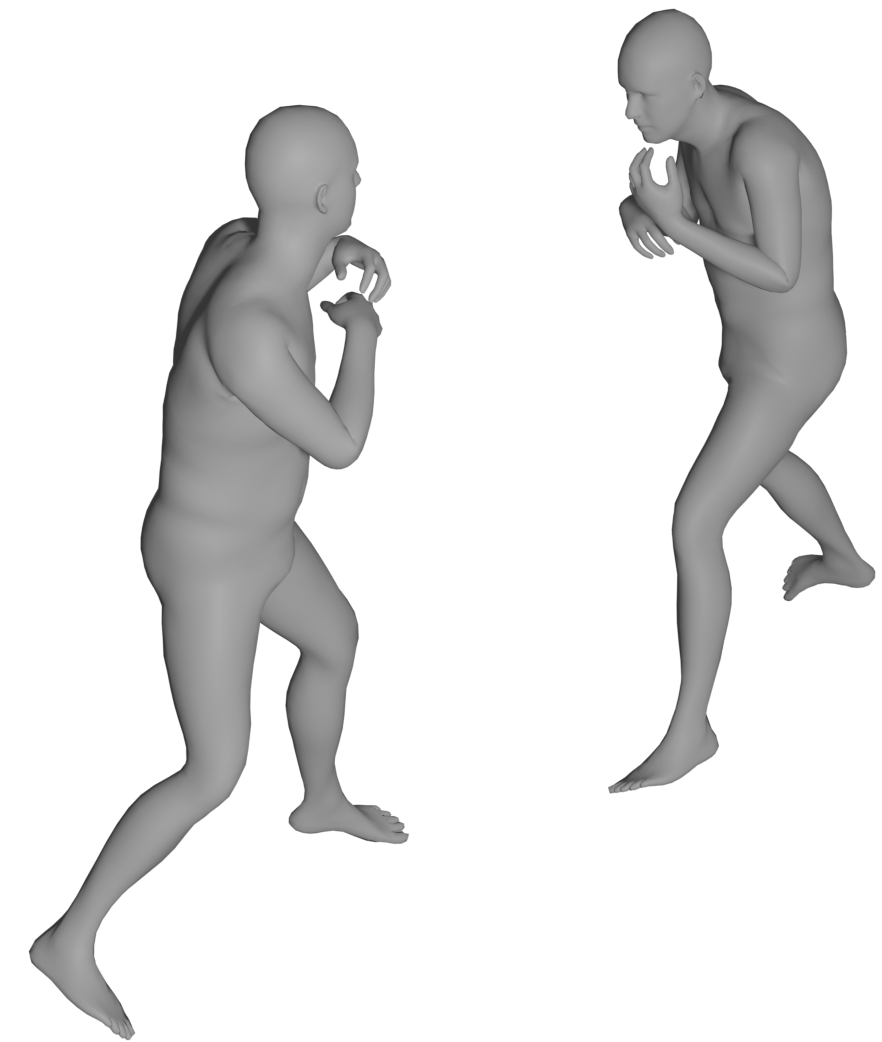
\includegraphics[scale=0.2]{figures/smpl2.png}} 
\put(0.5,9){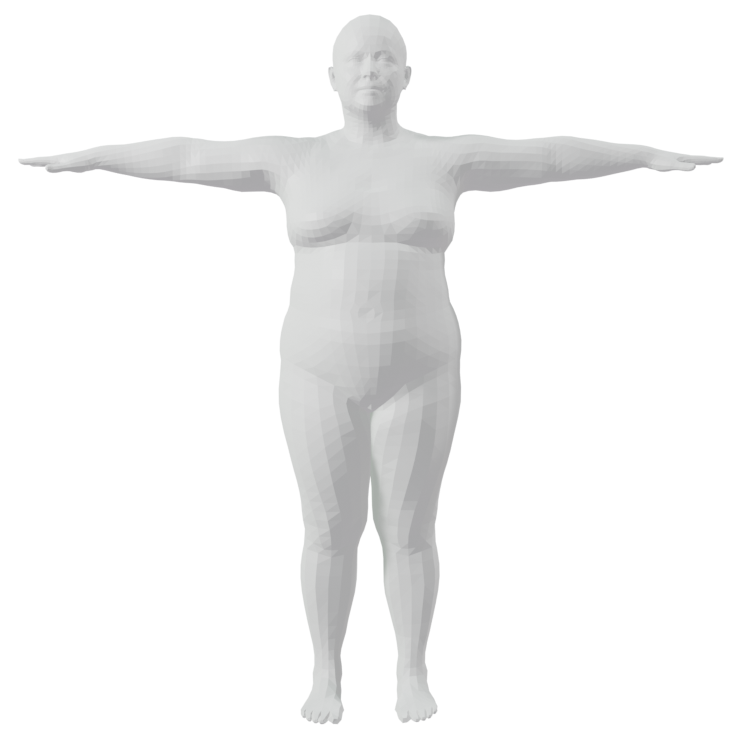
\includegraphics[scale=0.13]{figures/smpl-fat.png}} 
\put(0,0){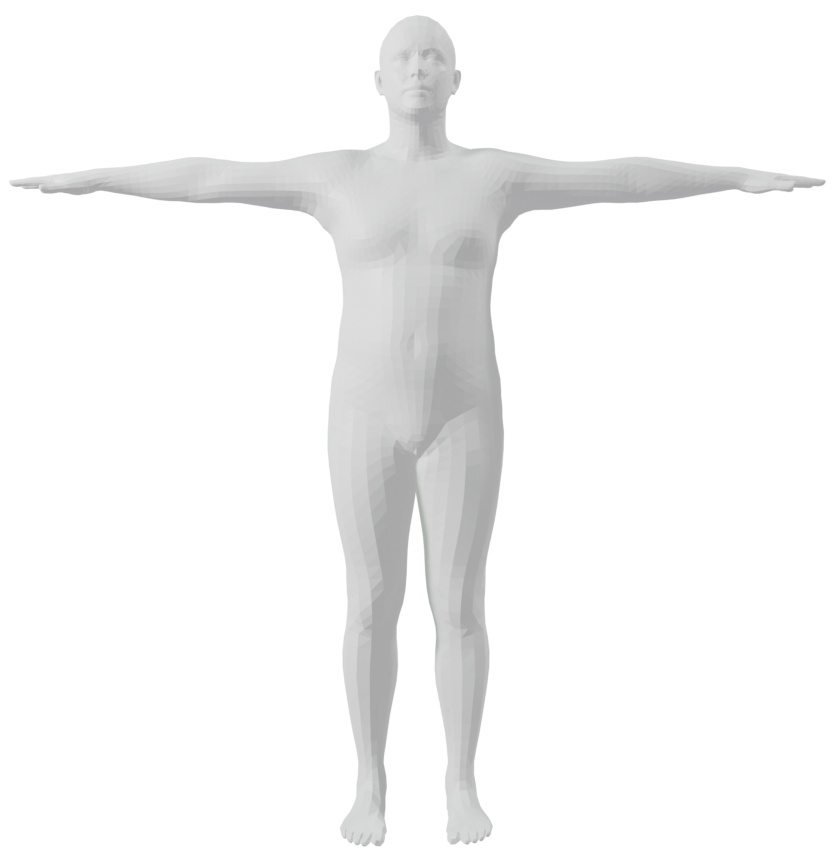
\includegraphics[scale=0.13]{figures/smpl-tall.png}}
\put(47.2,9){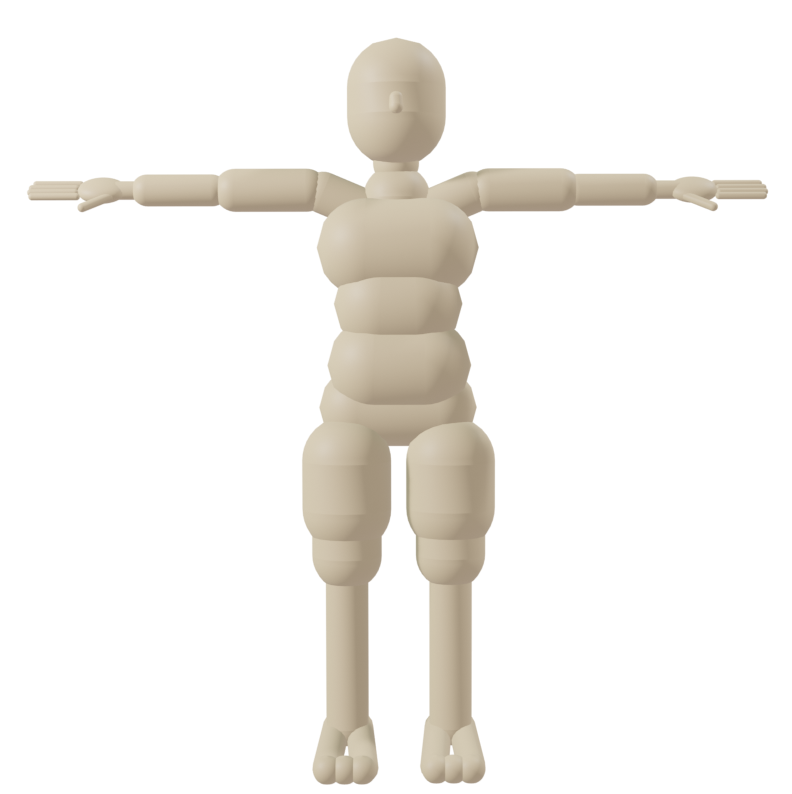
\includegraphics[scale=0.13]{figures/mujoco-fat.png}} 
\put(47,0){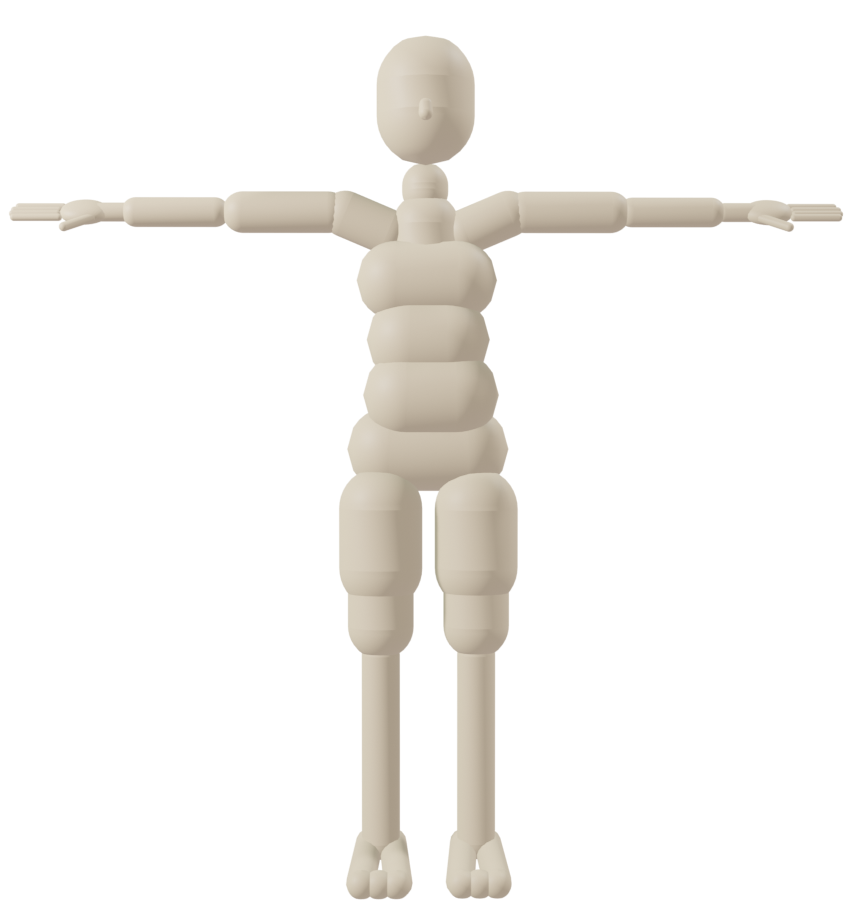
\includegraphics[scale=0.13]{figures/mujoco-tall.png}} 
\put(93,2){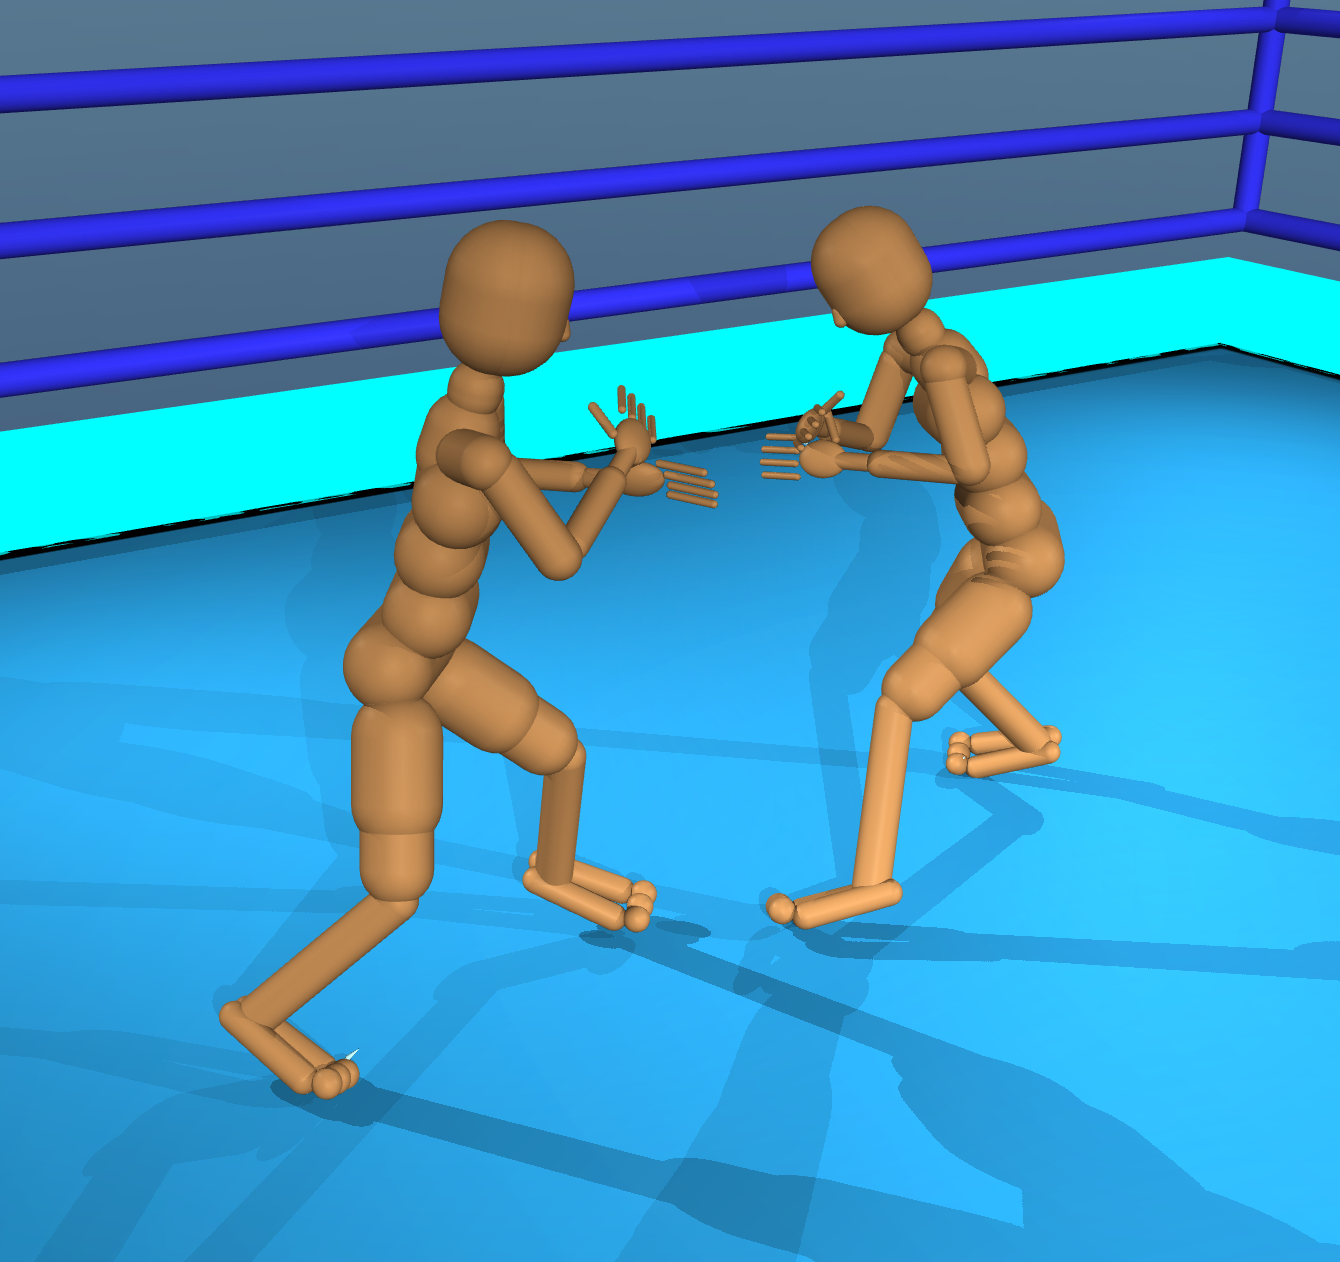
\includegraphics[scale=0.28]{figures/final.png}} 
\vspace{35pt}
\end{overpic}\\

\fontsize{36}{42}\selectfont The pipeline begins with generating bounding boxes ($\mathbf{bboxes}$) and robust tracking ($\mathrm{id}$) for each individual in the scene. These tracking results are used to produce 2D poses ($\mathbf{J}_\text{2D}$) using ViTPose~\cite{xu2022vitpose}. The triangulation process, produces smooth 3D keypoints ($\mathbf{J}_\text{3D}$). The kinematics optimization step incorporates the 2D and 3D keypoints, to create the SMPL parameters ($\theta$, $\beta$). The 3D relative joint positions ($\mathbf{p}$), initial pose state ($\mathbf{q}$) and velocity state ($\mathbf{v}$) of the humanoid (created using the physics body model generator), serve as a reference for a model predictive controller, which utilizes the iLQR optimizer~\cite{howell2022} to correct any artifacts in the motion.
}

\block[titleoffsetx=0cm, bodyoffsetx=0cm, titleoffsety=1cm, bodyoffsety=1cm]{Multi-frame Multi-view Tracking IDs}{
\begin{minipage}{\linewidth}
    \begin{itemize}
        \item \fontsize{29}{20}\selectfont \textbf{Tracking by Segmentation}: XMem creates short and long memory segments per view for consistent ID assignment across frames.~\cite{cheng2022xmem}
        \item \textbf{Epipolar Constraint-based ID Matching}: Matching across views using bounding box centroids and epipolar constraints.~\cite{wohler20093d}
        \item \textbf{Top-Down 2D Pose Estimation}: Using ViTpose keypoints are localized within bounding boxes for precise pose estimation.~\cite{xu2022vitpose}
    \end{itemize}
\end{minipage}
}

\block[titleoffsetx=0cm, bodyoffsetx=0cm, titleoffsety=1cm, bodyoffsety=1cm]{Weighted Triangulation and Filtering}{
\fontsize{38}{40}\selectfont
    Weighted triangulation estimates 3D keypoints from corresponding 2D keypoints across all $N$ cameras, accurately determining the 3D positions by solving the linear system:\vspace{20pt}
    \begin{tabular}{@{}p{0.55\textwidth}@{} p{0.43\textwidth}@{}}

        \innerblock[titlewidthscale=0.4, bodywidthscale=0.4]{Weighted Triangulation Formulation}{
        \begin{equation}
        \begin{bmatrix}
        \mu_{1} (\mathbf{P}_{11} - \mathrm{u}_1 \mathbf{P}_{31}) \\
        \mu_{1} (\mathbf{P}_{21} - \mathrm{v}_1 \mathbf{P}_{31}) \\
        \vdots \\
        \mu_{N} (\mathbf{P}_{1N} - \mathrm{u}_N \mathbf{P}_{3N}) \\
        \mu_{N} (\mathbf{P}_{2N} - \mathrm{v}_N \mathbf{P}_{3N}) \\
        \end{bmatrix}
        \begin{bmatrix}
        \mathrm{x} \\
        \mathrm{y} \\
        \mathrm{z} \\
        1
        \end{bmatrix}
        =
        \begin{bmatrix}
        0\\
        \vdots \\
        0
        \end{bmatrix} 
        \label{eq:tri}
        \end{equation}
        } &
        \vspace{-290pt}
        \hspace{-1100pt}
        \parbox[t]{0.55\linewidth}{
            $\mathbf{P}_{ij}$ extracts the $i$-th row of the projection matrix $\mathbf{P}_{j}$.  The average confidence of a 2D point for the current frame in camera $j$ is $\mu_{j}$. Higher confidence values give more weight to certain cameras.
            We use SVD to solve Eq.~\ref{eq:tri}. After triangulation, outliers are handled by interpolating and smoothing using cubic spline for each joint's trajectory. 
        }
    \end{tabular}
     \vskip -1.4cm

If triangulation fails, we apply an extended Kalman filter to estimate 3D keypoints using velocity, acceleration, and position constraints, ensuring reliable reconstructions from sparse, noisy 2D data.
}

\column{0.5}
\block[titleoffsety=0.25cm, bodyoffsety=0.25cm]{Kinematics Optimization}{
\fontsize{38}{40}\selectfont
Our kinematics optimization refines the SMPL model to minimize the difference between the provided 2D poses ($\mathbf{J}_{\text{2D}}$) from multiple views and 3D keypoints ($\mathbf{J}_{\text{3D}}$) obtained from triangulation. The process ensures temporal coherency and natural motion by incorporating smoothness and human motion priors. An LBFGS optimizer is used to solve the minimization problem, considering various loss terms, including 2D re-projection, 3D alignment, smoothness, and prior losses.
\vspace{0.4\baselineskip}

\fontsize{30}{36}\selectfont
\innerblock{Kinematics Optimization Formulation: 
$\min\limits_{\theta} w_1 \, \mathrm{L}_\text{2D} + w_2 \, \mathrm{L}_\text{3D} + w_3 \, \mathrm{L}_\text{reg} + w_4 \, \mathrm{L}_\text{smooth} + w_5 \, \mathrm{L}_{\text{GMM}} + w_6 \, \mathrm{L}_{\text{Vposer}}$}{
    \begin{multicols}{2}
        \begin{itemize}
            \item \textbf{2D Re-projection Loss}: Aligns the 3D joints with 2D joints using re-projection, weighted by confidence.\\ $\mathrm{L}_\text{2D} = \sum\limits_{\text{j} \in \text{$\mathcal{V}$}} \, \sum\limits_{\text{i} \in \text{$\mathbf{J}_{2D}$}} c_\text{j,i} \rho (\mathrm{J}_{\text{proj}_{j,i}} - \mathrm{J}_{2D_{j,i}})$ 
            \vspace{-0.39\baselineskip}
            \item \textbf{3D Alignment Loss}:  Minimizes the difference between predicted and actual 3D joint positions considering confidence. 
            \\ $\mathrm{L}_\text{3D} = \sum\limits_{\text{i} \in \text{$\mathbf{J}_{3D}$}} c_i \| \mathrm{J}_i(\theta, \beta) - \mathrm{J}_{3D,i}\|^2$
            \item \textbf{Smoothness Loss}: Ensures temporal consistency by minimizing differences in poses and vertices over time.\\
            $\mathrm{L}_{\text{smooth}} = \sum\limits_{t} \| \theta^t - \theta^{t-1} \|^2 + \| \mathcal{M}(\theta^t, \beta) - \mathcal{M}(\theta^{t-1}, \beta) \|^2$
            \vspace{-0.54\baselineskip}
            \item \textbf{Prior Loss}:  Guides the optimization towards natural poses using GMM and Vposer priors. \\ $\mathrm{L}_{\text{GMM}} = \frac{1}{N} \sum_{i=1}^{N} \text{GMM}(\theta_i, \beta), \quad \mathrm{L}_{\text{Vposer}} = \frac{1}{N} \sum_{i=1}^{N} (\text{z}(\theta_i)^{2})$
        \end{itemize}
    \end{multicols}
    \vspace{-0.39\baselineskip}
}
\vspace{-0.39\baselineskip}
}

\useblockstyle{blockred}

\block[titleoffsetx=0cm, bodyoffsetx=0cm, titleoffsety=1.23cm, bodyoffsety=1.23cm]{Physics Body Model Generator}{
\vspace{-0.39\baselineskip}
\fontsize{38}{40}\selectfont
   Our goal is to reconstruct the motion of \( K \) physics-based humanoids at each time step \( t \). The combined state is \( \mathbf{x}_t = (\mathbf{q}_t, \mathbf{v}_t) \), where \( \mathbf{q}_t \in \mathbb{R}^{63K} \) is the joint rotations vector, and \( \mathbf{v}_t \in \mathbb{R}^{62K} \) is the joint velocities vector. The 3D SMPL joint positions are \( \mathbf{p}_t \in \mathbb{R}^{21K} \). The vector \( \mathbf{q}_t \) uses minimal coordinates for joint rotations, while \( \mathbf{p}_t \) represents the 3D positions relative to the humanoid's body frame, which are used in optimization. We used the Mujoco~\cite{todorov2012mujoco} XML format for multi-humanoid modeling.
   \vspace{-0.39\baselineskip}
}
\useblockstyle{ets}
\block[titleoffsetx=0cm, bodyoffsetx=0cm, titleoffsety=1.3cm, bodyoffsety=1.3cm]{Multi-person Dynamics Optimization}{
\vspace{-0.39\baselineskip}
\fontsize{38}{40}\selectfont
The iLQR algorithm~\cite{howell2022} optimizes a control trajectory \(\mathbf{u}_{0:T}\) by minimizing the cost function. The reference positions. $\mathbf{p}_{t}$ and velocities $\mathbf{v}_t$ are extracted from the kinematics optimization at each frame $t$, and the trajectory optimization is "warm-started" using control parameters $\mathbf{u}_{t-1}$ from the previous frame. The control is updated iteratively as \(\Delta\mathbf{u}_t = \mathbf{K}_t\Delta\mathbf{x}_t + \alpha \mathbf{k}_t\), with \(\mathbf{K}_t\) and \(\mathbf{k}_t\) refined until convergence.
\vspace{-0.3\baselineskip}
\fontsize{30}{36}\selectfont
\innerblock[titlewidthscale=1, bodywidthscale=1]{Dynamics Optimization Formulation: $ \min\limits_{\mathbf{u}_{0:T}} \sum\limits_{t\in [0,T]} w_1 \mathrm{L_{\text{reg},t}} + w_2 \mathrm{L}_{\text{p},t} + w_3 \mathrm{L}_{\text{v},t} + w_4 \mathrm{L}_{\text{collision},t}$}{
\begin{multicols}{2}
    \setlength{\itemsep}{0pt} % Remove space between items
\begin{itemize}
    \item \textbf{Position Loss}: Minimizes the difference between predicted and actual 3D joint positions in each short horizon. \\
    $\mathrm{L}_{\text{p},t} = \sum\limits_{\text{i} \in \text{$\mathbf{J}_\text{3D}$}} \| \mathrm{p}_\text{i,t} - \mathrm{J}_\text{3D,i,t}\|^2$  
    \vspace{-0.4\baselineskip}
    \item \textbf{Velocity Loss}: Minimizes the difference between predicted and actual 3D joint velocities in each short horizon.\\  
    $\mathrm{L}_{\text{v},t} = \sum\limits_{\text{i} \in \text{$\mathbf{J}_{3D}$}} c_i \| \mathrm{v}_\text{i,t} - \mathrm{v}_{3D,i,t}\|^2$
\end{itemize}
    \begin{itemize}
        \item \textbf{Collision Loss}: The collision term penalizes the penetration between the geoms of different humanoids.  \\
        $\mathrm{L}_{\text{collision},t} = \sum\limits_{\text{i\in{1\dots M}}} \sum\limits_{\text{j\in{1\dots M}}} \max(0, \epsilon - \text{dist}(G_{1_i}, G_{2_j}))$
        \item \textbf{Regularization Loss}: Prevent sudden changes in control input. $\mathrm{L}_{\text{reg},t} = \|\mathbf{u}_t\|^2$
    \end{itemize}
\end{multicols}
\vspace{-0.39\baselineskip}
}
\vspace{-0.5\baselineskip}
}

\block[titlewidthscale=0.385, bodywidthscale=0.385, titleoffsetx=-17.5cm, bodyoffsetx=-17.5cm, titleoffsety=1.2cm, bodyoffsety=1.2cm]{
Discussion and Future Works}{
\vspace{-0.39\baselineskip}
\fontsize{38}{40}\selectfont

    \parbox{0.54\linewidth}{
        We created a 10-hour dataset of boxing motions to develop a model for generating intelligent VR responses.
    }
    \vspace{-0.5\baselineskip}
}
\block[titlewidthscale=0.1, bodywidthscale=0.1, titleoffsetx=-3cm, bodyoffsetx=-3cm, titleoffsety=8.4cm, bodyoffsety=8.4cm]{Video}{
\vspace{-0.7\baselineskip}

\hspace{-0.5\baselineskip}
    \qrcode[height=4.5cm]{https://youtu.be/agatO-jXEZk}
\vspace{-0.6\baselineskip}
}
\block[titlewidthscale=0.49, bodywidthscale=0.49, titleoffsetx=14.5cm, bodyoffsetx=14.5cm, titleoffsety=8.4cm, bodyoffsety=8.4cm]{Visualization}{
\vspace{-0.7\baselineskip}
    \begin{tikzpicture}[inner sep=0pt, outer sep=0pt]

        % Define CMYK color for arrows
        \definecolor{myCyan}{cmyk}{1, 0.2, 0, 0.2}

        % First image
        \node (img1) at (0,0) {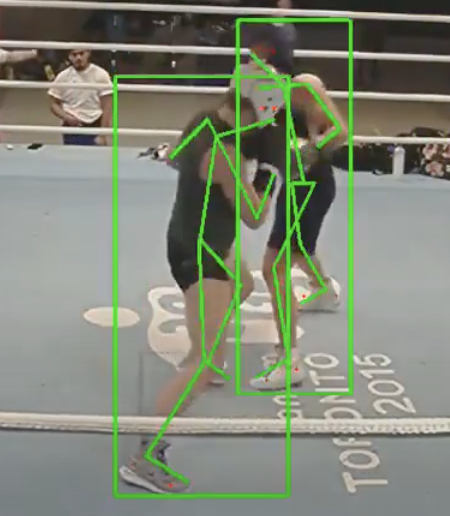
\includegraphics[width=5cm, height=4.65cm]{figures/image20.png}};
        
        % Second image to the right of the first
        \node (img2) at (2,0) {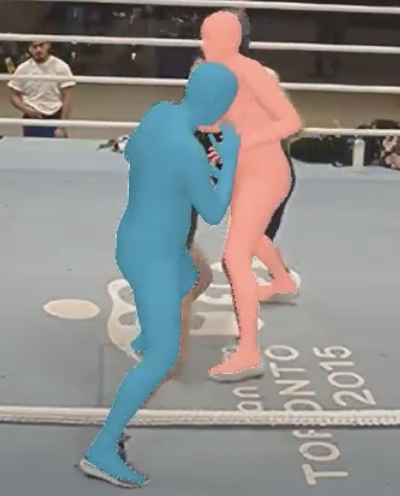
\includegraphics[width=5cm, height=4.65cm]{figures/image21.png}};
        
        % Third image to the right of the second
        \node (img3) at (4,0) {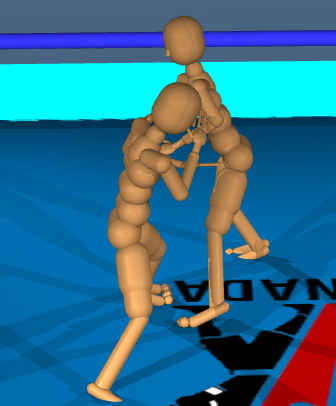
\includegraphics[width=5cm, height=4.65cm]{figures/image23.png}};
        
        % Fourth image to the right of the third
        \node (img4) at (6,0) {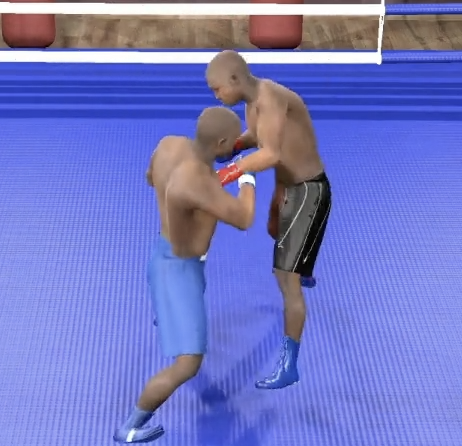
\includegraphics[width=5cm, height=4.65cm]{figures/image19.png}};
        
        % Fancy arrows between images with labels higher and in CMYK color
        \draw[-{Latex[length=6mm, width=3mm, inset=0.5mm]}, line width=2mm, color=myCyan] 
            (img1.east) -- node[above=6mm, font=\tiny\bfseries] {$\mathbf{J}_\text{2D}$} (img2.west);
        \draw[-{Latex[length=6mm, width=3mm, inset=0.5mm]}, line width=2mm, color=myCyan] 
            (img2.east) -- node[above=6mm, font=\tiny\bfseries] {$(\theta, \beta)$} (img3.west);
        \draw[-{Latex[length=6mm, width=3mm, inset=0.5mm]}, line width=2mm, color=myCyan] 
            (img3.east) -- node[above=6mm, font=\tiny\bfseries] {$(\mathbf{q}, \tau)$} (img4.west);

    \end{tikzpicture}
\vspace{-1.7\baselineskip}
}
   

\block[titleoffsetx=0cm, bodyoffsetx=0cm, titleoffsety=1.3cm, bodyoffsety=1.3cm]{References}{   \vspace{-0.6\baselineskip}
        \renewcommand*{\bibfont}{\small} 
        \printbibliography[heading=none]
   \vspace{-0.68\baselineskip}
}
\end{columns}

% Node for images at the bottom of the poster
\node [above right,
    text=titlefgcolor,
    outer sep=0pt,
    minimum width=\textwidth,
    minimum height=2cm, % Increased height for more space
    align=left,
    fill=titlebgcolor, inner sep=2mm] at (bottomleft) { % Increased inner sep
    \hspace{-1900pt}
    
\begin{tikzpicture}[scale=0.3] % Increased scale for the envelope
        \draw (0,0) -- (1,0) -- (1,0.7) -- (0,0.7) -- cycle; % Envelope outline
        \draw (0,0.7) -- (0.5,0.35) -- (1,0.7); % Envelope flap
    \end{tikzpicture}

    \href{mailto:hfa.zadeh.k@gmail.com}{\Large hfa.zadeh.k@gmail.com} % Increased font size
    \hspace{150pt} % Adjusted spacing
    \Large Linked
    \tikz[baseline=(i.base)]\node[fill=blue, rounded corners=0.5ex, text=white, inner sep=0.3ex, outer sep=0pt, minimum width=0pt, minimum height=0pt](i) {\large in}; % Increased font and inner sep
    
    \href{https://ca.linkedin.com/in/hosseinfeiz}{\Large Hossein Feiz} % Increased font size
    \hspace{150pt} % Adjusted spacing
    
    \tikz[baseline=(i.base)]\node[fill=black, rounded corners=0.5ex, text=white, font=\bfseries\sffamily\Large, inner sep=0.4ex, outer sep=0pt, minimum width=0pt, minimum height=0pt](i) {X}; % Increased font size and inner sep
    
    \href{https://x.com/hosseinfeiz1}{\Large hosseinfeiz1} % Increased font size
};

\end{document}